\documentclass[a4paper, 12pt]{article}

% Document quality things
\usepackage[utf8]{inputenc}
\usepackage{microtype, xcolor}
\usepackage{csquotes}
\usepackage{url, hyperref}
\hypersetup{colorlinks=true, linkcolor=black, citecolor=black, urlcolor=blue}

% Image-related packages
\usepackage{graphicx}
%\usepackage{float}
% \graphicspath{{./gfx/}}
%\usepackage[font=small,skip=5pt]{caption}

% Setting margins
\usepackage[a4paper,bottom=2.5cm,top=2.5cm,left=2.5cm,right=2.5cm]{geometry}
\renewcommand{\baselinestretch}{1.5} 

% Table helper packages
%\usepackage{multirow, multicol}
%\usepackage{makecell}
%\usepackage{array}
%\usepackage{tabularx} % Not needed currently, but has a few nice options
%\usepackage{wrapfig} % Floating figures/tables
\usepackage{booktabs}
\usepackage{longtable}

% Prevents spamming tedious newlines everywhere, also disables auto indentation, etc.
\usepackage[skip=0pt]{parskip}

\usepackage{titlesec}
\titleformat*{\section}{\normalsize\scshape}
\titleformat*{\subsection}{\normalsize\itshape}
\titlespacing{\section}{0pt}{12pt}{0pt}
\titlespacing{\subsection}{0pt}{12pt}{0pt}

\usepackage{tikz, pgfplots}
\pgfplotsset{compat=1.18}
\usetikzlibrary{automata, positioning, arrows}

% \usepackage{pdflscape, pdfpages}

\begin{document}
  \begin{center}
    {\large CS 342 - Project 2}\\
    Vedat Eren Arıcan - 22002643\\
  \end{center}

  Below are two plots whose data points were 10 iterations of varying average $\lambda$ values.
  \vspace{20pt}

  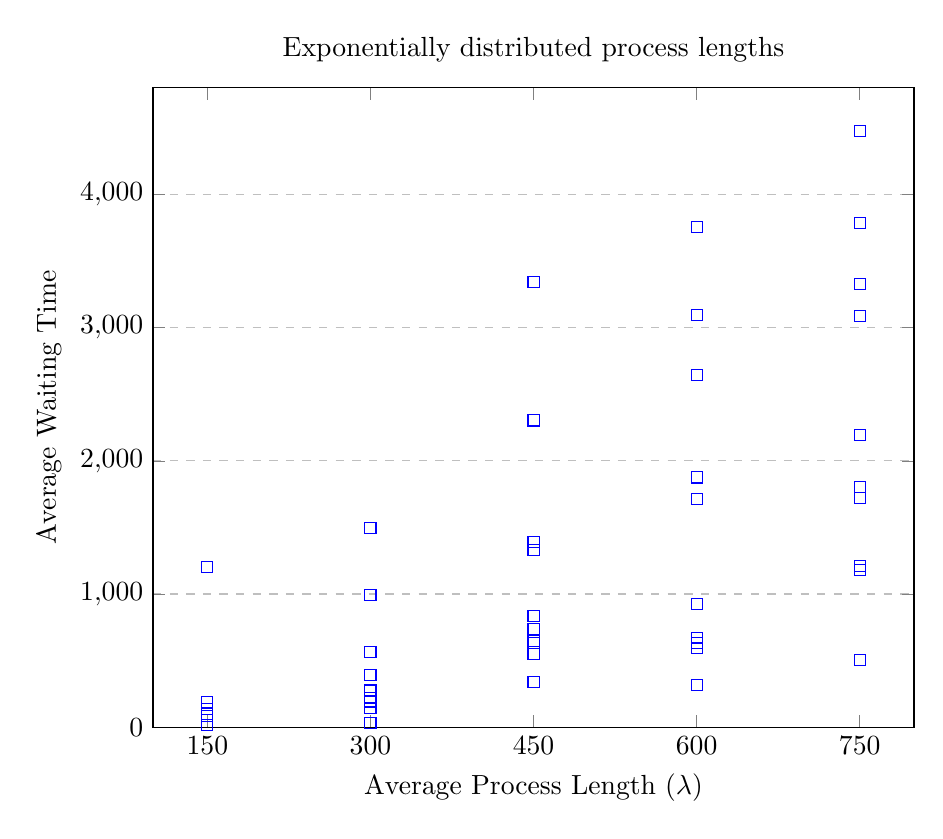
\begin{tikzpicture}
    \begin{axis}[
      title={Exponentially distributed process lengths},
      width=\textwidth - 25,
      xlabel={Average Process Length ($\lambda$)},
      ylabel={Average Waiting Time},
      xmin=100, xmax=800,
      ymin=0, ymax=4800,
      xtick={150,300,450,600,750},
      %ytick={0,20,40,60,80,100,120},
      ymajorgrids=true,
      grid style=dashed,
    ]

    \addplot[
        color=blue,
        only marks,
        mark=square,
      ]
      coordinates {
        (150,187)(150,84)(150,135)(150,14)(150,1205)(150,14)(150,16)(150,97)(150,85)(150,100)
        (300,275)(300,30)(300,145)(300,220)(300,391)(300,993)(300,565)(300,188)(300,1497)(300,199)
        (450,835)(450,735)(450,341)(450,647)(450,1328)(450,3343)(450,1388)(450,2303)(450,549)(450,632)
        (600,629)(600,925)(600,671)(600,2641)(600,596)(600,1875)(600,318)(600,3096)(600,1710)(600,3755)
        (750,3088)(750,3330)(750,1209)(750,4479)(750,1177)(750,1721)(750,2194)(750,3787)(750,1805)(750,504)
      };
        
    \end{axis}
  \end{tikzpicture}

  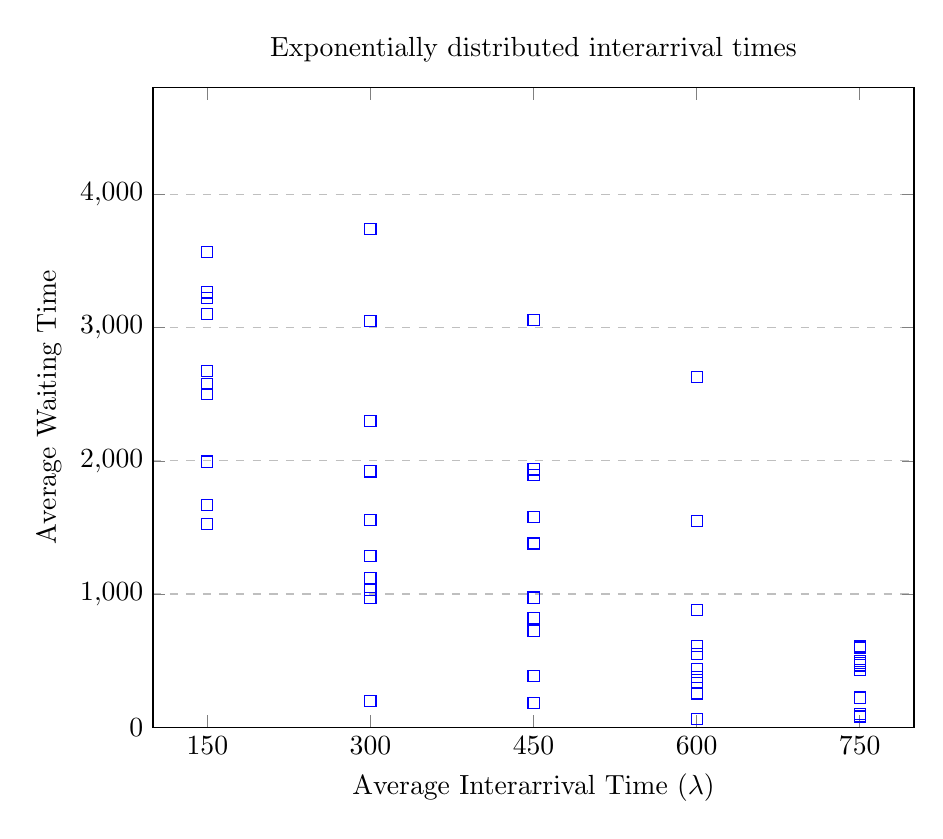
\begin{tikzpicture}
    \begin{axis}[
      title={Exponentially distributed interarrival times},
      width=\textwidth - 25,
      xlabel={Average Interarrival Time ($\lambda$)},
      ylabel={Average Waiting Time},
      xmin=100, xmax=800,
      ymin=0, ymax=4800,
      xtick={150,300,450,600,750},
      %ytick={0,20,40,60,80,100,120},
      ymajorgrids=true,
      grid style=dashed,
    ]

    \addplot[
        color=blue,
        only marks,
        mark=square,
      ]
      coordinates {
        (150,3264)(150,2677)(150,2502)(150,1666)(150,3569)(150,1994)(150,3220)(150,2579)(150,3104)(150,1528)
        (300,1119)(300,971)(300,1558)(300,1033)(300,194)(300,2298)(300,1920)(300,3741)(300,1287)(300,3051)
        (450,1935)(450,1379)(450,721)(450,3060)(450,1580)(450,181)(450,816)(450,973)(450,1896)(450,382)
        (600,329)(600,379)(600,2630)(600,253)(600,548)(600,877)(600,608)(600,437)(600,62)(600,1547)
        (750,430)(750,495)(750,100)(750,598)(750,607)(750,85)(750,481)(750,222)(750,463)(750,75)
      };
        
    \end{axis}
  \end{tikzpicture}

  \vspace{30pt}

  We can conclude that as process lengths increase, there is a trend of reaching higher limits of average waiting times.
  However, it was also observed that the majority of data points still remain relatively small, most likely
  as a result of the CFS algorithm.

  As for the interarrival times, the same trend was visible in opposite direction.
  The waiting times decrease as the arrival of the next process gets later, since the runqueue has
  less processes to swap between. Again, the data points are kept relatively close, likely thanks to CFS.

\end{document}

